\documentclass{article}
\usepackage{gnuplot-lua-tikz}
\usepackage{tikz}
\usepackage{pgfplots}
\begin{document}
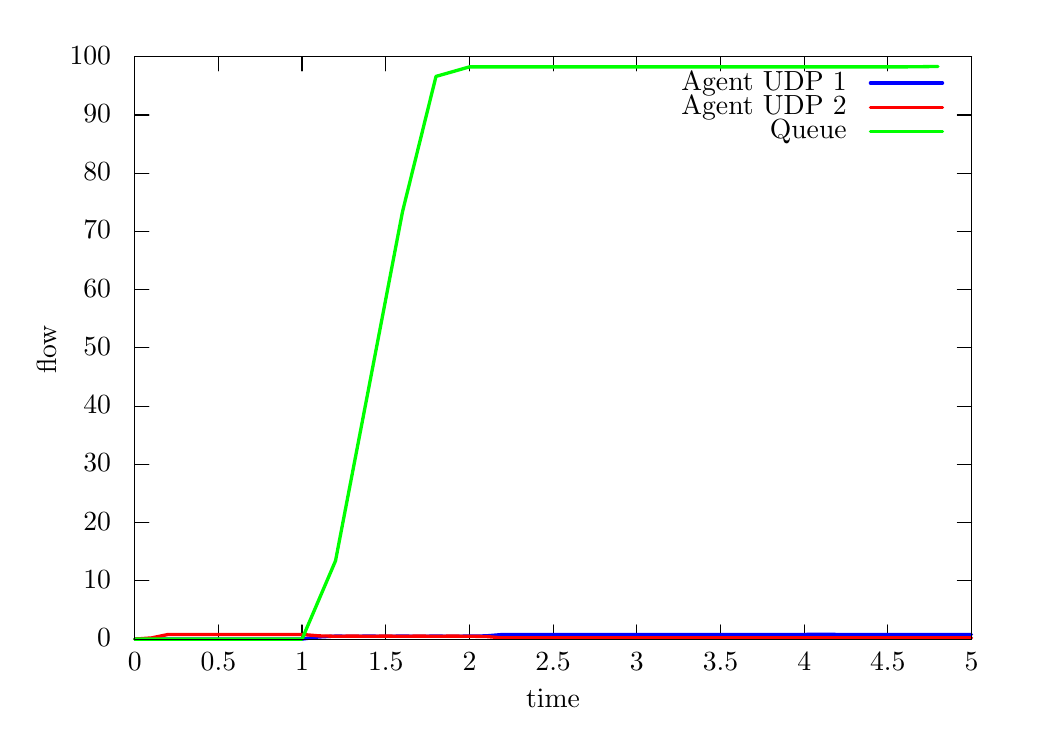
\begin{tikzpicture}[gnuplot]
%% generated with GNUPLOT 5.0prc2 (Lua 5.1; terminal rev. 99, script rev. 100)
%% mar. 03 nov. 2015 12:41:46 CET
\path (0.000,0.000) rectangle (12.500,8.750);
\gpcolor{rgb color={0.000,0.000,0.000}}
\gpsetlinetype{gp lt border}
\gpsetlinewidth{1.00}
\draw[gp path] (1.320,0.985)--(1.500,0.985);
\draw[gp path] (11.947,0.985)--(11.767,0.985);
\node[gp node right] at (1.136,0.985) {$0$};
\draw[gp path] (1.320,1.725)--(1.500,1.725);
\draw[gp path] (11.947,1.725)--(11.767,1.725);
\node[gp node right] at (1.136,1.725) {$10$};
\draw[gp path] (1.320,2.464)--(1.500,2.464);
\draw[gp path] (11.947,2.464)--(11.767,2.464);
\node[gp node right] at (1.136,2.464) {$20$};
\draw[gp path] (1.320,3.204)--(1.500,3.204);
\draw[gp path] (11.947,3.204)--(11.767,3.204);
\node[gp node right] at (1.136,3.204) {$30$};
\draw[gp path] (1.320,3.943)--(1.500,3.943);
\draw[gp path] (11.947,3.943)--(11.767,3.943);
\node[gp node right] at (1.136,3.943) {$40$};
\draw[gp path] (1.320,4.683)--(1.500,4.683);
\draw[gp path] (11.947,4.683)--(11.767,4.683);
\node[gp node right] at (1.136,4.683) {$50$};
\draw[gp path] (1.320,5.423)--(1.500,5.423);
\draw[gp path] (11.947,5.423)--(11.767,5.423);
\node[gp node right] at (1.136,5.423) {$60$};
\draw[gp path] (1.320,6.162)--(1.500,6.162);
\draw[gp path] (11.947,6.162)--(11.767,6.162);
\node[gp node right] at (1.136,6.162) {$70$};
\draw[gp path] (1.320,6.902)--(1.500,6.902);
\draw[gp path] (11.947,6.902)--(11.767,6.902);
\node[gp node right] at (1.136,6.902) {$80$};
\draw[gp path] (1.320,7.641)--(1.500,7.641);
\draw[gp path] (11.947,7.641)--(11.767,7.641);
\node[gp node right] at (1.136,7.641) {$90$};
\draw[gp path] (1.320,8.381)--(1.500,8.381);
\draw[gp path] (11.947,8.381)--(11.767,8.381);
\node[gp node right] at (1.136,8.381) {$100$};
\draw[gp path] (1.320,0.985)--(1.320,1.165);
\draw[gp path] (1.320,8.381)--(1.320,8.201);
\node[gp node center] at (1.320,0.677) {$0$};
\draw[gp path] (2.383,0.985)--(2.383,1.165);
\draw[gp path] (2.383,8.381)--(2.383,8.201);
\node[gp node center] at (2.383,0.677) {$0.5$};
\draw[gp path] (3.445,0.985)--(3.445,1.165);
\draw[gp path] (3.445,8.381)--(3.445,8.201);
\node[gp node center] at (3.445,0.677) {$1$};
\draw[gp path] (4.508,0.985)--(4.508,1.165);
\draw[gp path] (4.508,8.381)--(4.508,8.201);
\node[gp node center] at (4.508,0.677) {$1.5$};
\draw[gp path] (5.571,0.985)--(5.571,1.165);
\draw[gp path] (5.571,8.381)--(5.571,8.201);
\node[gp node center] at (5.571,0.677) {$2$};
\draw[gp path] (6.634,0.985)--(6.634,1.165);
\draw[gp path] (6.634,8.381)--(6.634,8.201);
\node[gp node center] at (6.634,0.677) {$2.5$};
\draw[gp path] (7.696,0.985)--(7.696,1.165);
\draw[gp path] (7.696,8.381)--(7.696,8.201);
\node[gp node center] at (7.696,0.677) {$3$};
\draw[gp path] (8.759,0.985)--(8.759,1.165);
\draw[gp path] (8.759,8.381)--(8.759,8.201);
\node[gp node center] at (8.759,0.677) {$3.5$};
\draw[gp path] (9.822,0.985)--(9.822,1.165);
\draw[gp path] (9.822,8.381)--(9.822,8.201);
\node[gp node center] at (9.822,0.677) {$4$};
\draw[gp path] (10.884,0.985)--(10.884,1.165);
\draw[gp path] (10.884,8.381)--(10.884,8.201);
\node[gp node center] at (10.884,0.677) {$4.5$};
\draw[gp path] (11.947,0.985)--(11.947,1.165);
\draw[gp path] (11.947,8.381)--(11.947,8.201);
\node[gp node center] at (11.947,0.677) {$5$};
\draw[gp path] (1.320,8.381)--(1.320,0.985)--(11.947,0.985)--(11.947,8.381)--cycle;
\node[gp node center,rotate=-270] at (0.246,4.683) {flow};
\node[gp node center] at (6.633,0.215) {time};
\node[gp node right] at (10.479,8.047) {Agent UDP 1};
\gpcolor{rgb color={0.000,0.000,1.000}}
\gpsetlinewidth{3.00}
\draw[gp path] (10.663,8.047)--(11.579,8.047);
\draw[gp path] (1.320,0.985)--(1.533,0.985)--(1.745,0.985)--(1.958,0.985)--(2.170,0.985)%
  --(2.383,0.985)--(2.595,0.985)--(2.808,0.985)--(3.020,0.985)--(3.233,0.985)--(3.445,0.985)%
  --(3.658,1.012)--(3.870,1.023)--(4.083,1.021)--(4.296,1.023)--(4.508,1.021)--(4.721,1.023)%
  --(4.933,1.021)--(5.146,1.023)--(5.358,1.021)--(5.571,1.023)--(5.783,1.026)--(5.996,1.044)%
  --(6.208,1.044)--(6.421,1.044)--(6.634,1.044)--(6.846,1.044)--(7.059,1.044)--(7.271,1.044)%
  --(7.484,1.044)--(7.696,1.044)--(7.909,1.044)--(8.121,1.044)--(8.334,1.044)--(8.546,1.044)%
  --(8.759,1.044)--(8.971,1.044)--(9.184,1.044)--(9.397,1.044)--(9.609,1.044)--(9.822,1.044)%
  --(10.034,1.047)--(10.247,1.044)--(10.459,1.044)--(10.672,1.044)--(10.884,1.044)--(11.097,1.044)%
  --(11.309,1.044)--(11.522,1.044)--(11.734,1.044)--(11.947,1.044);
\gpcolor{rgb color={0.000,0.000,0.000}}
\node[gp node right] at (10.479,7.739) {Agent UDP 2};
\gpcolor{rgb color={1.000,0.000,0.000}}
\draw[gp path] (10.663,7.739)--(11.579,7.739);
\draw[gp path] (1.320,0.985)--(1.533,1.000)--(1.745,1.044)--(1.958,1.044)--(2.170,1.044)%
  --(2.383,1.044)--(2.595,1.044)--(2.808,1.044)--(3.020,1.044)--(3.233,1.044)--(3.445,1.044)%
  --(3.658,1.026)--(3.870,1.021)--(4.083,1.023)--(4.296,1.021)--(4.508,1.023)--(4.721,1.021)%
  --(4.933,1.023)--(5.146,1.021)--(5.358,1.023)--(5.571,1.021)--(5.783,1.018)--(5.996,1.000)%
  --(6.208,1.000)--(6.421,1.000)--(6.634,1.000)--(6.846,1.000)--(7.059,1.000)--(7.271,1.000)%
  --(7.484,1.000)--(7.696,1.000)--(7.909,1.000)--(8.121,1.000)--(8.334,1.000)--(8.546,1.000)%
  --(8.759,1.000)--(8.971,1.000)--(9.184,1.000)--(9.397,1.000)--(9.609,1.000)--(9.822,1.000)%
  --(10.034,1.000)--(10.247,1.000)--(10.459,1.000)--(10.672,1.000)--(10.884,1.000)--(11.097,1.000)%
  --(11.309,1.000)--(11.522,1.000)--(11.734,1.000)--(11.947,1.000);
\gpcolor{rgb color={0.000,0.000,0.000}}
\node[gp node right] at (10.479,7.431) {Queue};
\gpcolor{rgb color={0.000,1.000,0.000}}
\draw[gp path] (10.663,7.431)--(11.579,7.431);
\draw[gp path] (1.320,0.985)--(1.745,0.985)--(2.170,0.985)--(2.595,0.985)--(3.020,0.985)%
  --(3.445,0.985)--(3.870,1.979)--(4.296,4.195)--(4.721,6.414)--(5.146,8.131)--(5.571,8.252)%
  --(5.996,8.252)--(6.421,8.252)--(6.846,8.252)--(7.271,8.252)--(7.696,8.252)--(8.121,8.252)%
  --(8.546,8.252)--(8.971,8.252)--(9.397,8.252)--(9.822,8.252)--(10.247,8.252)--(10.672,8.252)%
  --(11.097,8.252)--(11.522,8.257);
\gpcolor{rgb color={0.000,0.000,0.000}}
\gpsetlinewidth{1.00}
\draw[gp path] (1.320,8.381)--(1.320,0.985)--(11.947,0.985)--(11.947,8.381)--cycle;
%% coordinates of the plot area
\gpdefrectangularnode{gp plot 1}{\pgfpoint{1.320cm}{0.985cm}}{\pgfpoint{11.947cm}{8.381cm}}
\end{tikzpicture}
\end{document}
%% gnuplot variables
